\documentclass{article}
\usepackage[utf8]{inputenc}
\usepackage{amsmath}
\usepackage{amsfonts}
\usepackage{amssymb}
\usepackage{minted}
\usepackage{graphicx}
\graphicspath{ {img/} }
\usepackage{titlesec}
\usepackage[a4paper,margin=1in,footskip=0.25in]{geometry}
\usepackage{fancyhdr}
\pagestyle{fancy}
%basic page layout

%draw finite state machine
\usepackage{tikz}
\usetikzlibrary{arrows,automata}
\newcommand{\hwnumber}{1}
%header and footer settings
\lhead{Gen IMS II Homework \hwnumber}
\chead{Yiping Deng}
\rhead{\today}

\titlelabel{\thetitle\enspace}

\begin{document}
\title{Gen IMS II Homework \hwnumber}
\author{Yiping Deng}
\maketitle
\thispagestyle{fancy}
\section*{Task 1}
\subsection*{a)}
Starting from the basic formula, we have:
\begin{align}
    Q &= CV_C \\
    \frac{dQ}{dt} &= i \\
    V_S &= V_C + V_R \\
    V_R &= iR
\end{align}
Using the formula above, we can differentiate (1) with respect to t
\begin{align}
    \frac{dQ}{dt} &= C \frac{dV_C}{dt} = i \\
\end{align}
Thus, equation (4) can be substituted using (5)
\begin{align}
    V_R &= R C \frac{dV_C}{dt}
\end{align}
Plug into (3), we have first order seperable ODE
\begin{align}
    RC \frac{dV_C}{dt} + V_C = V_S
\end{align}
\subsection*{b)}
We can solve (9) by seperation of variable:
\begin{align}
    RC \frac{dV_C}{V_C - V_S} &= -dt
\end{align}
Integrate both side, we have
\begin{align}
    ln(V_C + V_S) &= -\frac{t}{RC} + constant
\end{align}
Take the exponential function on both side
\begin{align}
    V_C - V_S = B e^{-\frac{t}{RC}}
\end{align}
Also, plug-in the initial condition, we have:
\begin{align}
    0  - V_S &= B \\
    B &= -V_S
\end{align}
The solution is:
\begin{align}
    V_C(t) &= V_S - V_S e^{-\frac{t}{RC}} \\
    A &= V_S \\
    B &= -V_S \\
    \lambda &= -\frac{1}{RC} \\
\end{align}

\subsection*{c)}
Using the following python code, we can generate a graph
\begin{minted}{python}
import numpy as np
import matplotlib.pyplot as plt
import math

def graph(formula, points):
    x = points
    y = formula(x)
    plt.plot(x, y)
    plt.show()

graph(lambda t: 10 - 10 * np.exp(-t/(1000 * 100* 10**-6)), np.linspace(0, 0.7, 200))
\end{minted}
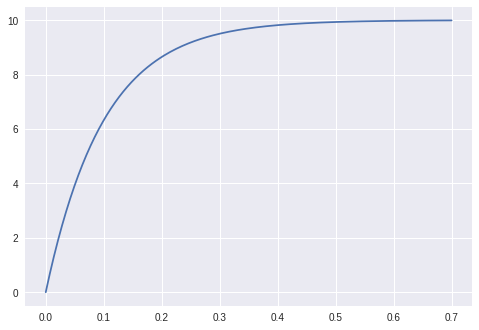
\includegraphics{plot.png}
\end{document}
